%% !TEX TS-program = pdflatex
%% !TEX encoding = UTF-8 Unicode
%\documentclass[11pt]{article} % use larger type; default would be 10pt
%\usepackage[utf8]{inputenc} % set input encoding (not needed with XeLaTeX)
%
%%%% PAGE DIMENSIONS
%\usepackage{geometry} % to change the page dimensions
%\geometry{a4paper} % or letterpaper (US) or a5paper or....
%
%%%% PACKAGES
%\usepackage{qtree} % Tree support
%\usepackage{graphicx} % support the \includegraphics command and options
%\usepackage{wrapfig} % Figure wrapping
%% \usepackage[parfill]{parskip} % Activate to begin paragraphs with an empty line rather than an indent
%\usepackage{booktabs} % for much better looking tables
%\usepackage{array} % for better arrays (eg matrices) in maths
%\usepackage{paralist} % very flexible & customisable lists (eg. enumerate/itemize, etc.)
%\usepackage{verbatim} % adds environment for commenting out blocks of text & for better verbatim
%\usepackage{subfig} % make it possible to include more than one captioned figure/table in a single float
%\usepackage{url}
%\usepackage{enumerate}
%\usepackage{cleveref}  %cites figures intelligently
%\usepackage{import} % document structuring
%\usepackage{float}  %These two ensure that table position follows text by specifcing {table}[H]
%\restylefloat{table}
%
%%CODE LISTINGS
%\usepackage{color}
%\usepackage{listings}
%
%\lstset{
%	tabsize=4,
%%	language=matlab,
%        	basicstyle=\scriptsize,
%%     	upquote=true,
%       	aboveskip={\baselineskip},
%        	columns=fixed,
%        	showstringspaces=false,
%        	extendedchars=true,
%        	breaklines=true,
%	prebreak = \raisebox{0ex}[0ex][0ex]{\ensuremath{\hookleftarrow}},
%	frame=single,
%        	showtabs=false,
%        	showspaces=false,
%        	showstringspaces=false,
%        	identifierstyle=\ttfamily,
%        	keywordstyle=\color[rgb]{0,0,1},
%        	commentstyle=\color[rgb]{0.133,0.545,0.133},
%        	stringstyle=\color[rgb]{0.627,0.126,0.941},
%	language=C++
%}
%
%%%% HEADERS & FOOTERS
%\usepackage{fancyhdr} % This should be set AFTER setting up the page geometry
%\pagestyle{fancy} % options: empty , plain , fancy
%\renewcommand{\headrulewidth}{0pt} % customise the layout...
%\lhead{}\chead{}\rhead{}
%\lfoot{}\cfoot{\thepage}\rfoot{}
%
%%%% SECTION TITLE APPEARANCE
%\usepackage{sectsty}
%\allsectionsfont{\sffamily\mdseries\upshape} % (See the fntguide.pdf for font help)
%%\ttfamily
%%\sffamily\mdseries\upshape
%\rmfamily
%\usepackage{titlesec}
%%\titleformat{\subsection}[runin]{\mdseries\bf}{\thesubsection}{1em}{}
%%\titleformat{\subsubsection}[runin]{\mdseries\bf\underline\large}{\thesubsection}{1 em}{\vspace{-5 pt}}
%
%\usepackage{footbib}
%
%% (This matches ConTeXt defaults)
%
%%%% ToC (table of contents) APPEARANCE
%\usepackage[nottoc,notlof,notlot]{tocbibind} % Put the bibliography in the ToC
%\usepackage[titles,subfigure]{tocloft} % Alter the style of the Table of Contents
%\renewcommand{\cftsecfont}{\rmfamily\mdseries\upshape}
%\renewcommand{\cftsecpagefont}{\rmfamily\mdseries\upshape} % No bold!
%\newcommand{\tab}{\hspace*{2em}}
%
%\begin{document}
%%%% END Article customizations

\vspace{-20pt}
\part{User Interfaces}
\vspace{-20pt}
\section{GUI Map}\label{guimap}
\begin{figure}[H]
	\vspace{-20pt}
	\begin{center}
		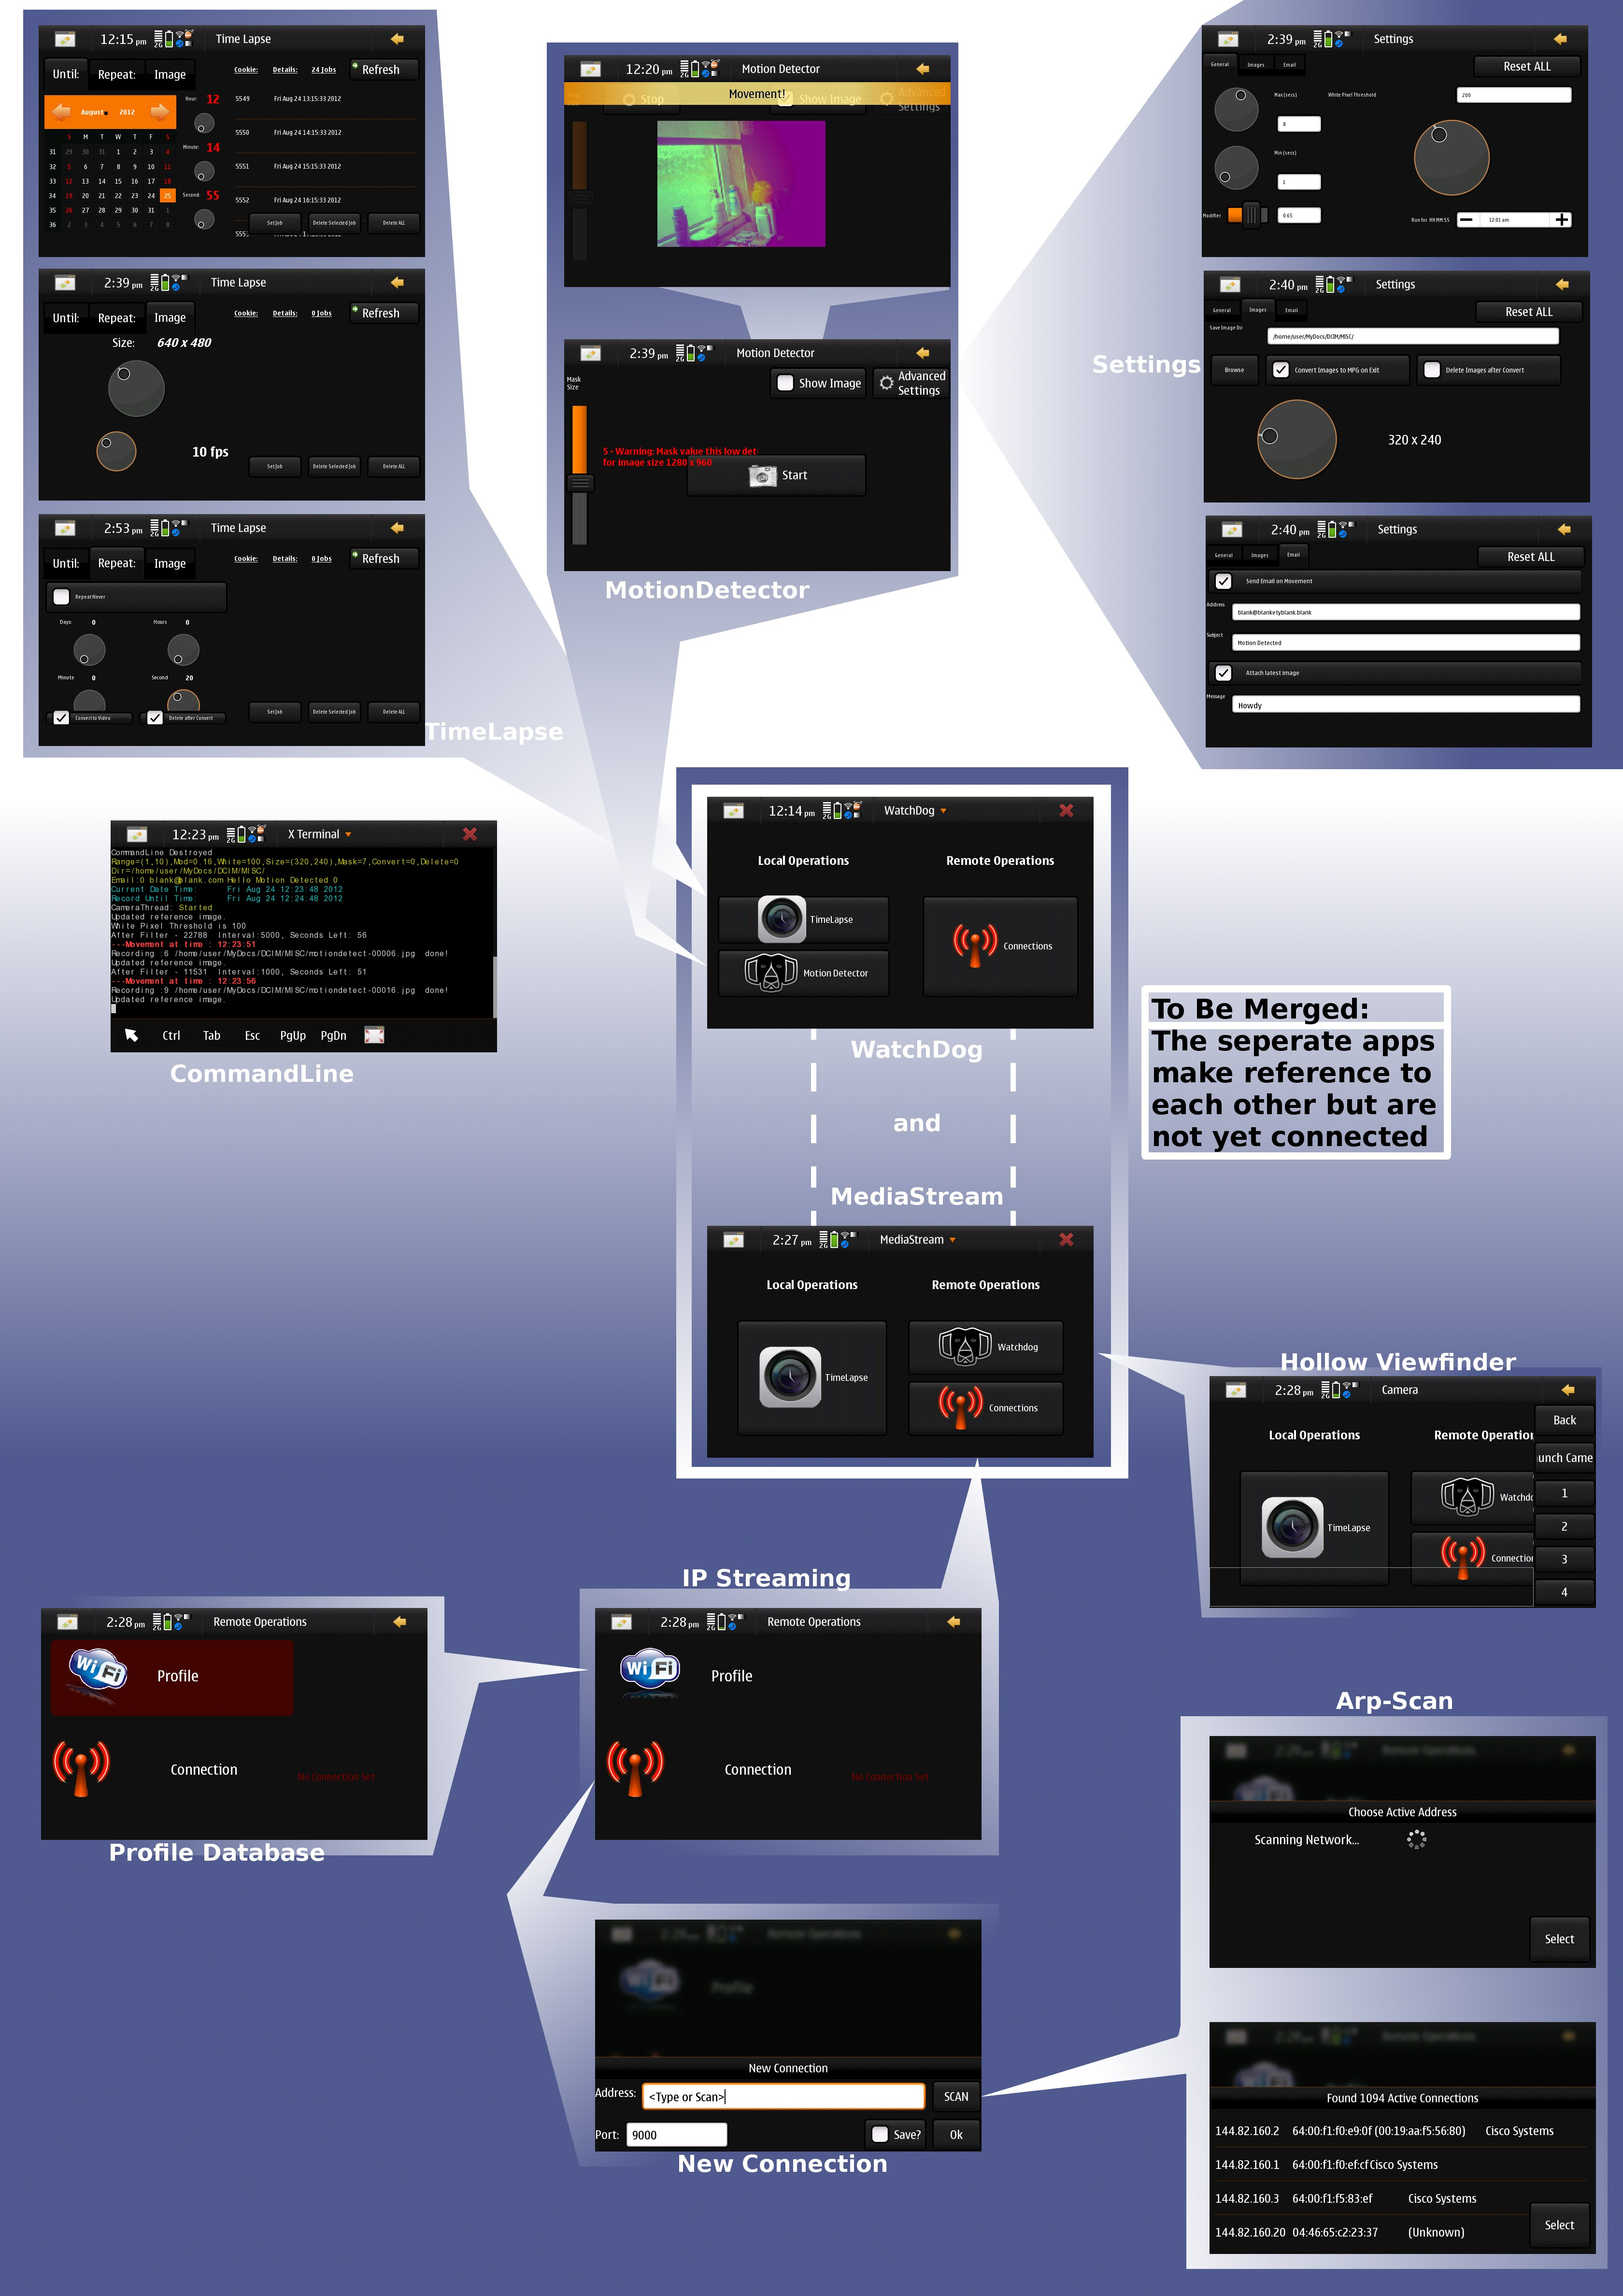
\includegraphics[width=1.1\textwidth]{../images/map}
		\label{img:map}
	\end{center}
	\vspace{-30pt}
	\caption{Map of every UI window for both WatchDog(motiondetector and timelapse) and Mediastream(IP streaming), and how they link to each other.}
\end{figure}

\section{Widgets}

Widgets in Qt can be very difficult to work with, and certain common operations such as applying styles, or inserting images, or inserting animated gifs, or even getting the UI to slide from window to the next without getting dangling pointers can be slightly difficult to implement.

To find out how I overcame these problems please consult page~\pageref{widgetstuff} in the Other Implementation section of the Appendix.

\section{Window management and Maemo5 Stacked Windows}
Unlike iPhone and Android user interfaces, Maemo does not automatically slide between different windows when initiated, but instead creates a new window and shifts view to it, whilst the previous window still exists. 

This isn't much of a problem if the user is solely using the one app because the user will not notice it. However Maemo was one the first platforms to support multitasking windows for mobiles, and so if the user has multiple windows open at any one time, then switching between windows suddenly becomes tediousy difficult as there now many windows open at any one time.

One solution is to simply call QMainindow::hide() or QMainWindow::show() between different windows so that only one window is shown at any one time, but this is inelegant, and ultimately leads to confusion of how many windows are being hidden which can waste memory if those windows are not being used.

To overcome this I trawled through the forums and came across Maemo5StackedWindow. This is a window property that enables sliding transitions and works only on the Maemo5 device. To enable it one must place the following in the constructor in {\it every} window of the project:
\begin{lstlisting}
#ifdef Q_WS_MAEMO_5
    this->setAttribute(Qt::WA_Maemo5StackedWindow);
    this->setWindowFlags(Qt::Window);
#endif
\end{lstlisting}

This solves the sliding window transition problem and saves window space when multitasking. However it does still waste memory, since the window(s) that were switched from are still active, but just hidden.

To overcome this problem I implemented pointer control
\subsection{Pointer Control}
In Qt, when creating a new Window (or any object), one can create it by simply calling 'new MyWindow(this)'. The this is an optional argument given to all windows which simply refers the child Window to the parent via a pointer. The child can perform very limited operations upon the parent window such as hide() or show() mentioned previously, but usually it is not used very much.

But how can the parent control the child? By pointers. Instead of creating a new window and throwing into the memory, the parent creates a {\it pointer} to the child window so that it knows exactly where it is and what to do with it. This is shown by calling:
'MyWindow *point = new MyWindow(this)'.

So now the parent can delete the child at any time it wants by simply calling the delete command, forcing the child window to be destroyed. This may seem slightly evil, but it is neccesary. Consider the followin situation:
\begin{enumerate}
\item User opens app, MainWindow pops up
\item User wants to access Motion Detector, so they select it and the MotionDetectorWindow slides into view
\item User wants to change a Setting within MotionDetector, so they press the Settings button and the SettingWindow slides into view. We now have 3 windows open and active (MainWindow, MotionDetectorWindow, and SettingsWindow).
\item User finishes setting Settings, and goes back to MotionDetector. An eager developer may choose to delete the SettingsWindow at this point since it is not being of any use, however a cautios developer may reason that the user may want to change another setting in the nearby future and so it would be easier to keep SettingsWindow in memory to delete and recreate it.
\item User finishes with MotionDetector and goes back to MainWindow. Again, it would be unwise to delete MotionDetectorWindow just in case the user goes back into it, and so it should remain in memory (along with SettingsWindow) to enable ease of access.
\item User wants to use TimeLapse function, so they now click on Timelapse button instead of MotionDetector button, and TimeLapse button slides into view. At {\it this} point there are now 4 windows open (MainWindow, MotionDetectorWindow, SettingsWindow, TimeLapseWindow) which is a {\it waste of memory} because the user is unlikely to use the MotionDetector while they are using TimeLapse. It is at this stage that a developer should {\it delete MotionDetectorWindow and SettingsWindow}. This will leave just two windows open (MainWindow and TimeLapseWindow) and save memory.
\end{enumerate}
The key underlying logic here is that when the user chooses TimeLapse functionality, all MotionDetector windows and subwindows are deleted, and vice versa (when the user chooses MotionDetector functionality, all TimeLapse windows and subwindows are deleted).

This may seem complicated, but it is rather trivial. The command 'delete settingsPointer' 
%HEERE KEEP WRITING




\section{Persisting data}
\subsection{QSettings}

%\end{document}